\section{Explainable AI 1}
What makes XAI difficult?:
\begin{enumerate}
    \item \textbf{The missingness problem:}
    
    How to properly define missingness
    \item \textbf{The correlation problem}
    
    How to tractably consider feature dependence
\end{enumerate}

\subsection{Nomenclature}
\begin{itemize}
    \item \textbf{Global:} Creating a summary of which features most influence predictions across all instances in a dataset, such as using SHAP to determine overall feature importance in a model
    \item \textbf{Surrogat:} Using a decision tree to approximate and explain a complex neural network model's behaviour by replicating its predictions
    \item \textbf{Attributions:} A heatmap that shows which pixel in an image contributed the most to a model's decision that the image contained a dog
    \item \textbf{Intrinsic:} A simple decision tree model used for classification where the splits and rules can be directly interpreted by humans
    \item \textbf{Local:} Analyzing why a specific instance of a loan application was approved or denied by examining factors unique to that case
    \item \textbf{Counterfactual:} Suggesting that if a loan applicant's income had been 5000\$ higher, thier loan would have been approved
    \item \textbf{Post hoc:} Using an XAI method explain predictions of a black-box model after the model has made a prediction
\end{itemize}

\subsection{Grad-CAM}
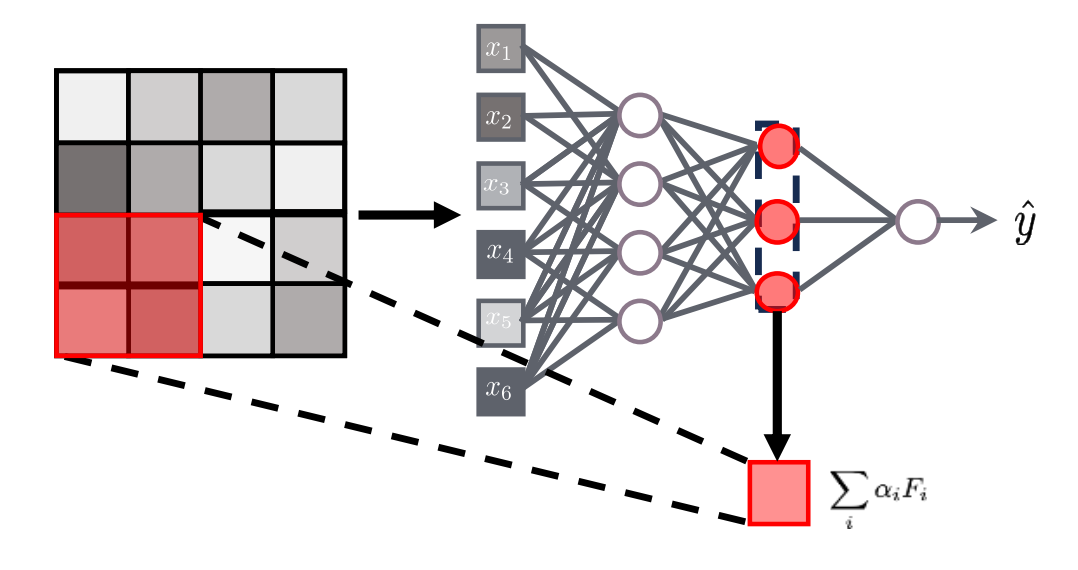
\includegraphics[width = \columnwidth]{figures/XAI1/GradCAM.png}

\subsection{interpreable}
\begin{itemize}
    \item These are simple models that we call white box models
    \item They require no fanccy XAI methods to interpret
    \item They are boring and make to many assumptions about the data
    \item They often from a vital component of some extravagant, powerful XAI methods, see LIME, Grad-CAM, SHAP, etc.
\end{itemize}
\subsection{Linear models}
\begin{figure}
    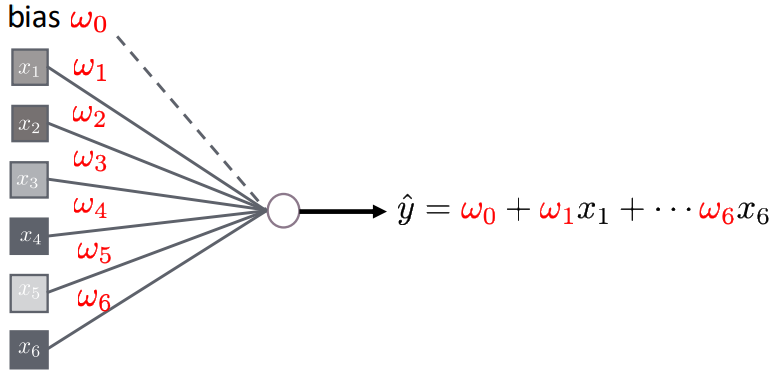
\includegraphics[width = 0.8\columnwidth]{figures/XAI1/LinearModels.png}
\end{figure}
Find optimal weights by minimizing MSE
\[
w^* = arg \min_{w_0 + \dots w_p}\sum_{i = 1}^{n}\left[y^{(i)}-\left(\mathbf{w}_0 + \sum_{j = 1}^{p}\mathbf{w}_j\mathbf{x}_j^{(i)}\right)\right]^2
\]

Interpretable metrics:
\begin{enumerate}
    \item Weights: The magnitude of a weight is proportional to the importance
    \item \(\text{R}^2\): Are the weights worth interpreting? i.e., is our model good?
    \item Adjusted \(\text{R}^2\): Improved to remove artifically inflating the fit by adding more features
\end{enumerate}
\subsubsection{Weights}
\begin{itemize}
    \item \(w = 0\):Weight of zero  means feature is unimportant because no matter the value of x, it gives the same result.
    \item \(w = 1\): Weight is larger, the y-value depends on the x-value. Negelcting the feature dependence will result in large errors
\end{itemize}
\subsubsection{\(\text{R}^2\)}
\begin{itemize}
    \item \(SEE\): Variance after the model has been fitted
    \item \(SST\): Natural amount of variance within the data
\end{itemize}
Exaplaining Variance with \(R^2 = 1 - SSE /SST\).
\[
SSE = \sum_{i = 1}^{n}\left(y^{(i)}-\hat{y}^{(i)}\right)^2 \qquad SST = \sum_{i = 1}^{n}\left(y^{(i)}-\overline{y}^{(i)}\right)^2
\]
\begin{itemize}
    \item \(R^2 = 1\): SST non-zero, SSE zero (perfect fit), weight are meaningfull
    \item \(R^2 < 1\): SST larger, SSE non-zero, weight are meaningfull
    \item \(R^2 \rightarrow 0\): Even though weight is large, the interpretability should not be trusted because the model does not capture the variance of the data. SEE and SST become comperable.
    \item \(R^2 < 0\): SEE bgger than SST,negative number, adverse model. Normally the fit would lie in the middle and thus result in smaller variance than the natural data variance
\end{itemize}
\subsubsection{Adjusted \(R^2\)}
Fix using the adjusted \(R^2\) metric:
\[
\overline{R}^2  = 1-(1-R^2)\frac{n-1}{n-p-1}
\]
p = \# of features, n = \# of instances.
Adjusted \(R^2\) penalizes for model complexity.

\subsubsection*{What happens if we have thousands of features}
\begin{itemize}
    \item Interpretability decreases
    \item Might even have more features than instances
\end{itemize}
Lasso regularization to introduce sparsity via the L1-norm.
\[
\mathcal{L} = \frac{1}{n}\sum_{i =1}^{n }\left(y^{(i)} - x_i^T\mathbf{w}\right)^2 + \lambda ||\mathbf{w}||_1
\]
Model not only wants to predict the data, but also wants to make the weights small.

\subsection{Decision-Trees}
Goal is to have good purity and loq complexity so tree model generalizes.

The idea of entropy can be used to achieve leaf purity
\[
H(D) = -\sum_{i = 1}^{k}p(C_i) \cdot log_2(p(C_i))
\]
\(C_i = \)black and white balls (2 classes)
\subsubsection{Grow a tree}
\begin{enumerate}
    \item For all possible features and splits calculate H
    \item Calculate weighted entropy for each split (larger purer states better)
    \[
    H_{after split} = \frac{|D_1|}{|D|}H(D_1) + \frac{|D_2|}{|D|}H(D_2)
    \]
    \item Calculate information gained from each split
    \[
    IG(D,A) = H(D) - H_{after split}
    \]
    \item Choose the feature and split with the highest information gain
\end{enumerate}
Reapeat until subsets are all pure, tree reaches max depth, minimum number of samples is reached.
\subsubsection{Feature importance}
\begin{itemize}
    \item \textbf{Feature split depth}: Features that are used higher up in the tree are more important
    \item \textbf{Feature split frequanzy}:
    Features that are used more often are more important
\end{itemize}
\subsubsection{Decision Trees XAI}
\begin{enumerate}
    \item \textbf{Feature importance} based on sum of information gain (Gini impurity)
    \item \textbf{Rule Extraction} for instance-level, intuitive explanations
    \item \textbf{Leaf Node Analysis}, look at distribution of features in a singel leaf
    \item \textbf{Counterfactual Explanations}, closest path resulting in different classification
\end{enumerate}
\subsubsection{Summary Decision Tree}
\begin{itemize}
    \item Trees are built using the idea of entropy
    \item The objectiv is to have leaf purity i.e., low entropy
    \item Features and splits are determined by maximizing information gain, this is the recipe to lower tree entropy
    \item Overfitting is prevented by hardcoding max tree depth, leaf purity threshold, etc.
    \item XAI local explanation by studying statistics of each group, counterfactuals by finding closest path that result in calss flips, rule based explanations for short trees, sum of weighted information gain for feature ranking
    \item Greedy or deterministic
\end{itemize}
\subsubsection{Summary Random forests}
\begin{itemize}
    \item Can be used for computationally cheap high performance outlier detection
    \item Is comparable to more complex methods such as single-class SVM and Gaussian mixture models
    \item Uses forests and random numbers
    \item Randomly select feature, randomly select split value
    \item Outliers are isolated in leaf nodes closer to the roots
    \item Aggregate results of isolating leaf depth is used to stabalize the random number
    \item Random numbers power the idea, and aggregates of many trees (forests) stabilize the results
\end{itemize}

\subsection{Plot based methods}
\subsubsection{Partial Dependency Plot (PDP)}
First order approximation of feature dependence. Assume features are uncorrelated

Procedure (Linearly):
\begin{enumerate}
    \item Select feature index to analyte (i = 2)
    \item Find unique values for this feature
    \item Order values of this features in ascending order
    \item Set feature \(i_0\) for all instances and calculate average
    \item Repeated this for \(i_1\) to \(i_n\) tracing out a curve
\end{enumerate}
Vectorize by replacing entire column with single featured value.
Problems: Examples might not be physical because features are most likely not independent.
\subsubsection{Individual Conditional Expectaion Plot (ICE)}
Second order approximation of feature dependency

Procedure (Linearly):
\begin{enumerate}
    \item Select feature index to analyte (i = 2)
    \item Find unique values for this feature
    \item Order values of this feature in ascending order
    \item Take single instance ans calculate BB-model output varying feature \(i\) over all its values to trace out a curve
    \item Reapeated for sub subsets
\end{enumerate}
\subsubsection{Summary}
\begin{itemize}
    \item Easy intuitive way to interpret a models dependency on a feature
    \item PDPs might hide critical information
    \item ICE shows more detail but are computationally expensive to calculate and can get visually overwhelming
    \item Both suffer from sparse data
    \item Both assume that features are independent, this might result in the generation of unrealistic data instance
\end{itemize}